\documentclass[12pt,fleqn]{article}\usepackage{../common}
\begin{document}


\begin{minted}[fontsize=\footnotesize]{python}
import pandas as pd
df = pd.read_csv('oilprice.csv',header=None,index_col=0)
pd.rolling_mean(df[1],40).plot()
plt.savefig('corr_01.png')
\end{minted}

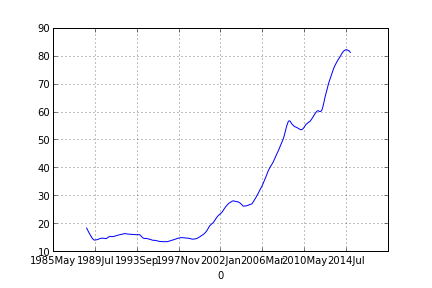
\includegraphics[height=6cm]{corr_01.png}


\begin{minted}[fontsize=\footnotesize]{python}
print len(list(pd.rolling_mean(df[1],80).dropna()))
\end{minted}

\begin{verbatim}
276
\end{verbatim}

\begin{minted}[fontsize=\footnotesize]{python}
import pandas as pd
import datetime
from dateutil.parser import parse
price = pd.read_csv('oilprice.csv',header=None,index_col=0)
prod = pd.read_csv('world.csv',parse_dates=True,index_col=0,sep=' ')
price.index = map(lambda x: datetime.datetime.strptime(x,'%Y%b'), price.index)
prod['price'] = price
print prod.price.corr(prod.oil)
\end{minted}

\begin{verbatim}
0.812066270665
\end{verbatim}

\begin{minted}[fontsize=\footnotesize]{python}
prod.plot()
plt.savefig('corr_02.png')
\end{minted}

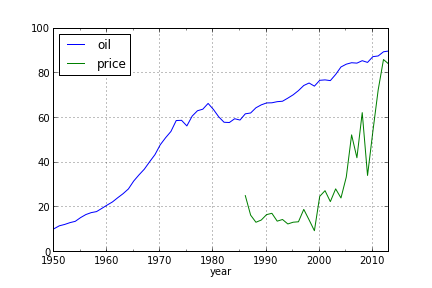
\includegraphics[height=6cm]{corr_02.png}

















\end{document}
